

\begin{figure}
  \centering
  \subfigure[�趨ģ�Ͳ���]{
    %\label{fig:subfig:a} %% label for first subfigure
    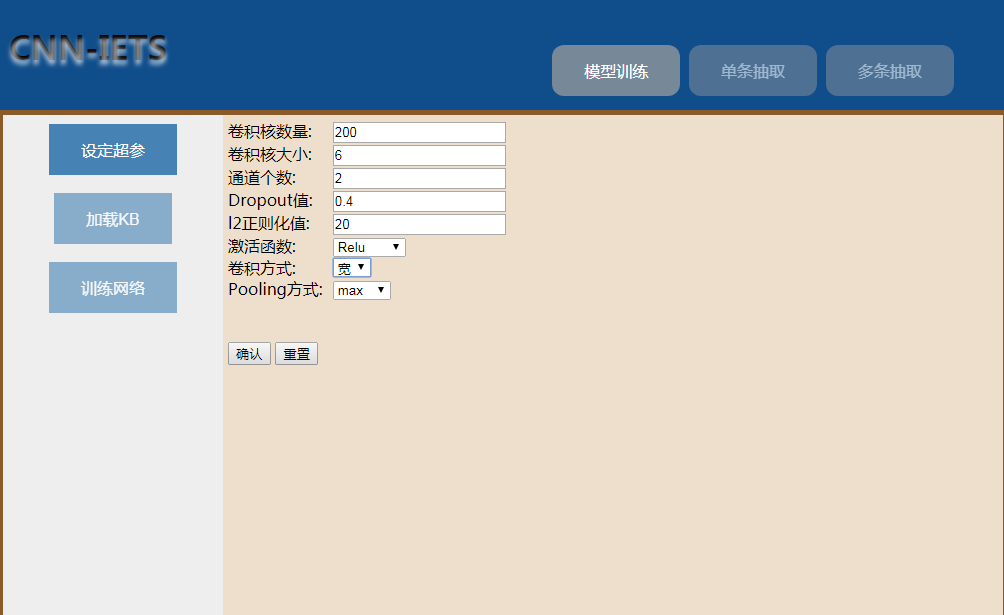
\includegraphics[width=3.5in]{../figures/chap04/set_model_para.png}
  }
  \subfigure[����֪ʶ��]{
    %\label{fig:subfig:a} %% label for first subfigure
    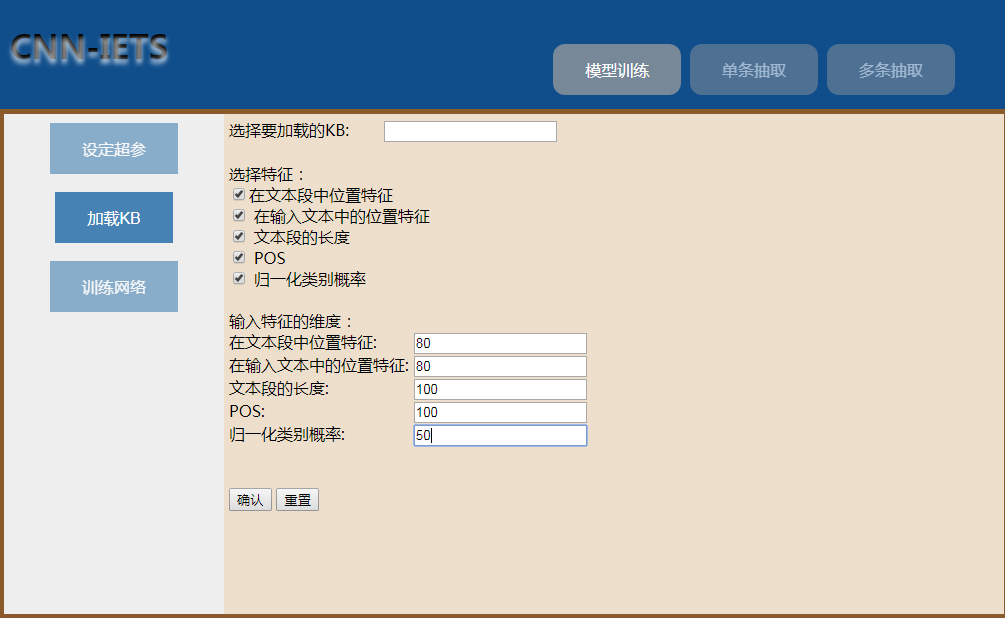
\includegraphics[width=3.5in]{../figures/chap04/load_kb.png}
  }
  \subfigure[ѵ��ģ��]{
    %\label{fig:subfig:a} %% label for first subfigure
    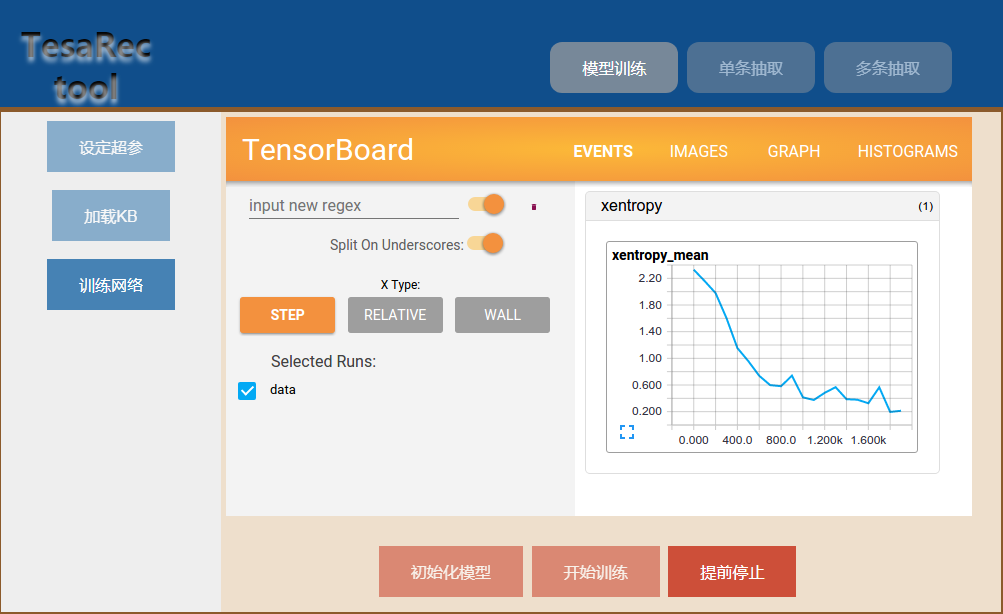
\includegraphics[width=3.5in]{../figures/chap04/train_model.png}
  }
  \caption{ģ�ͳ�ʼ����ѵ��}
  \label{fig:model_set_train} %% label for entire figure
\end{figure}


\begin{figure}
  \centering
  \subfigure[segment]{
    %\label{fig:subfig:a} %% label for first subfigure
    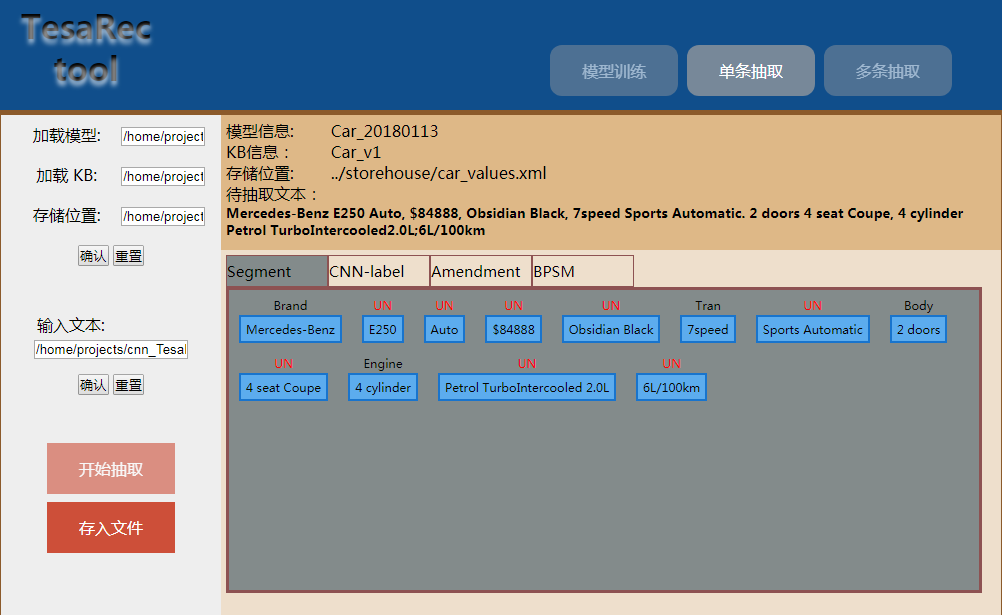
\includegraphics[width=3.4in]{../figures/chap04/segment-one.png}
  }
  \subfigure[cnn-label]{
    %\label{fig:subfig:a} %% label for first subfigure
    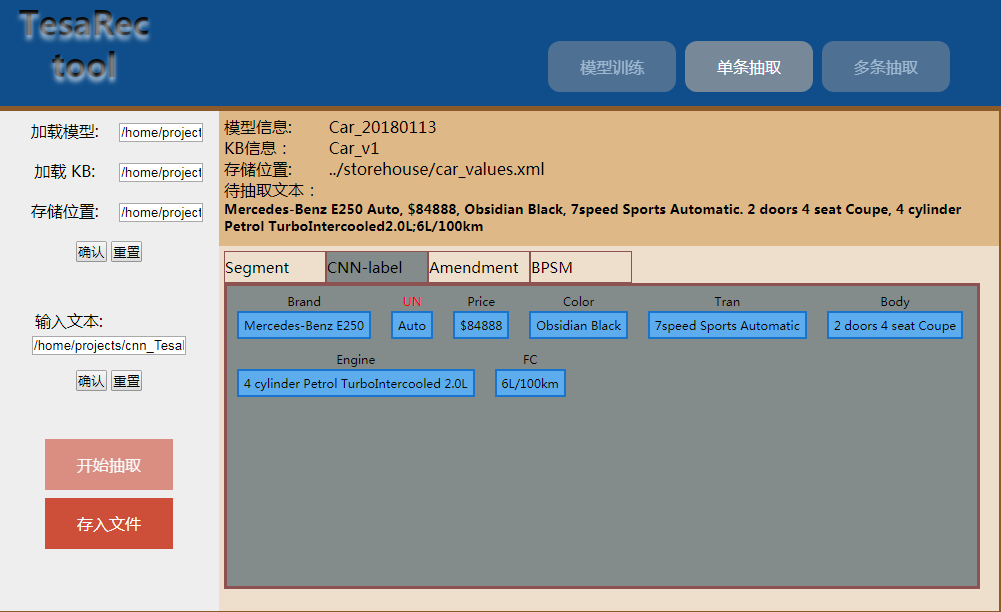
\includegraphics[width=3.5in]{../figures/chap04/cnn-label-one.png}
  }

  \subfigure[amendment]{
    %\label{fig:subfig:a} %% label for first subfigure
    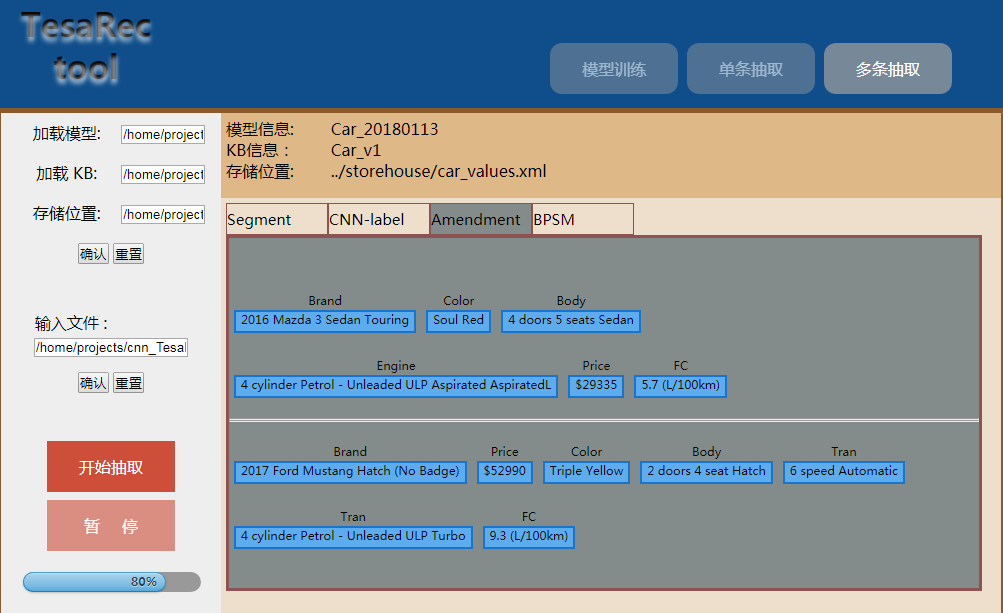
\includegraphics[width=3.5in]{../figures/chap04/amendment-mul.png}
  }
  \subfigure[BPSM]{
    %\label{fig:subfig:b} %% label for second subfigure
    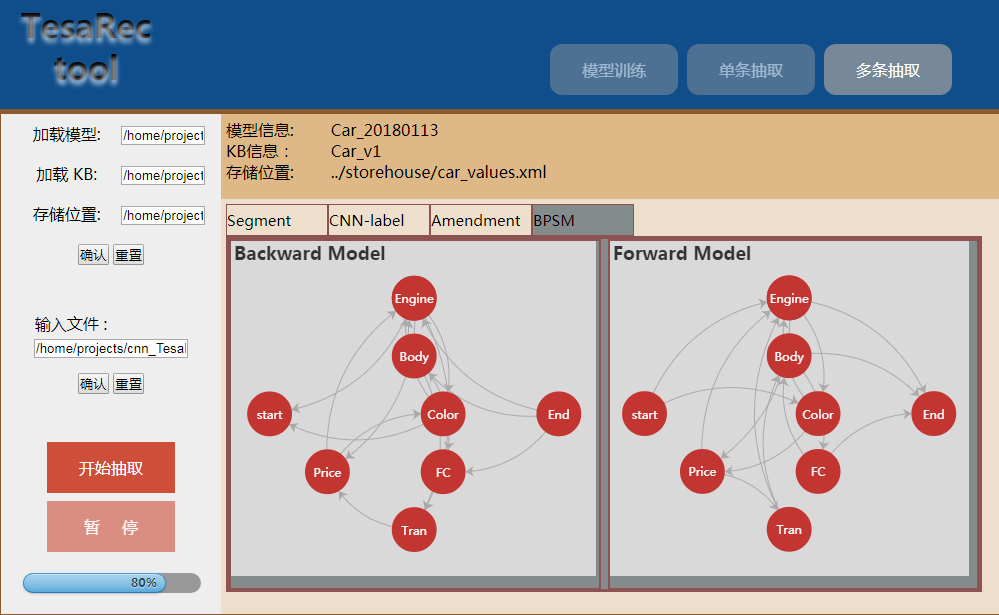
\includegraphics[width=3.5in]{../figures/chap04/BPSM-mul.png}
  }
  \caption{����һ����¼}
  \label{fig:one_record} %% label for entire figure
\end{figure}


\begin{figure}
  \centering
  \subfigure[segment]{
    %\label{fig:subfig:a} %% label for first subfigure
    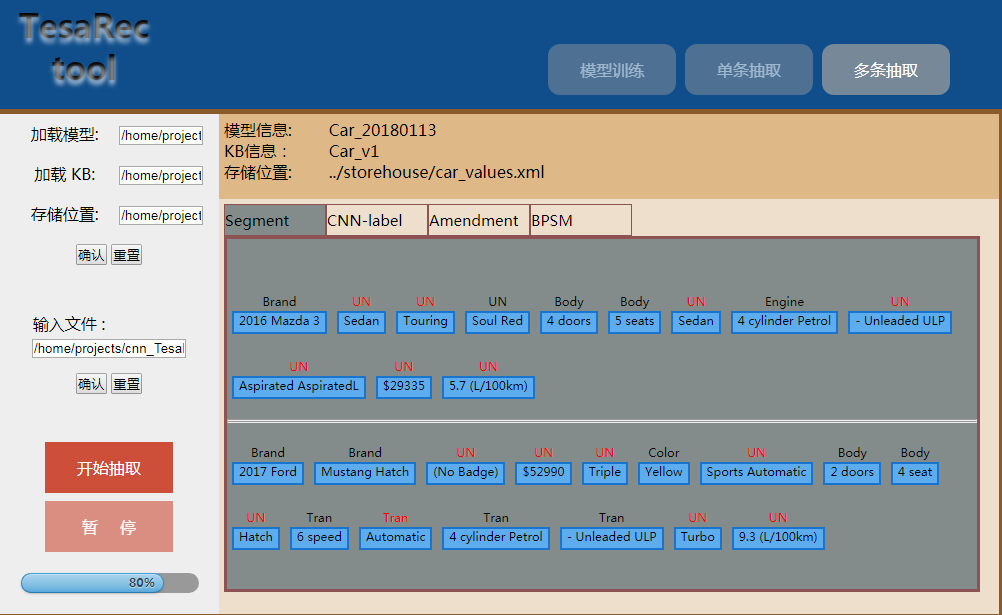
\includegraphics[width=3.5in]{../figures/chap04/segment-mul.png}
  }
  \subfigure[cnn-label]{
    %\label{fig:subfig:a} %% label for first subfigure
    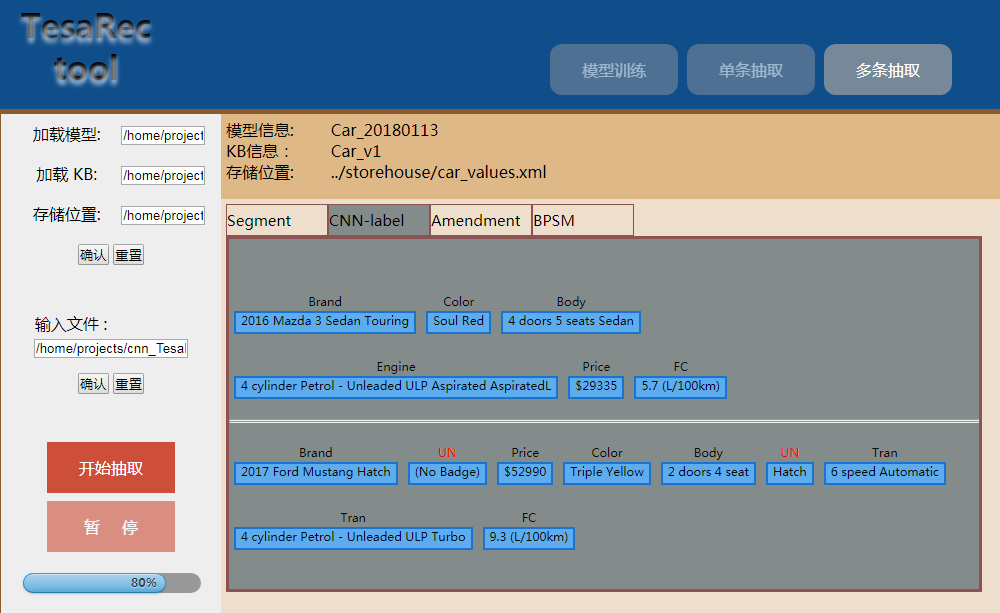
\includegraphics[width=3.5in]{../figures/chap04/cnn-label-mul.png}
  }

  \subfigure[amendment]{
    %\label{fig:subfig:a} %% label for first subfigure
    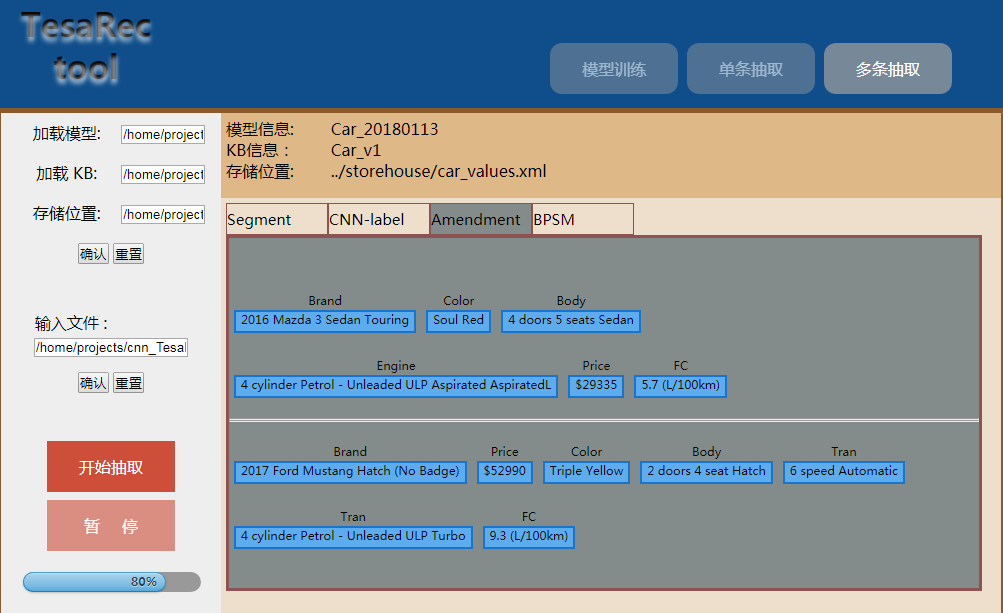
\includegraphics[width=3.5in]{../figures/chap04/amendment-mul.png}
  }
  \subfigure[BPSM]{
    %\label{fig:subfig:b} %% label for second subfigure
    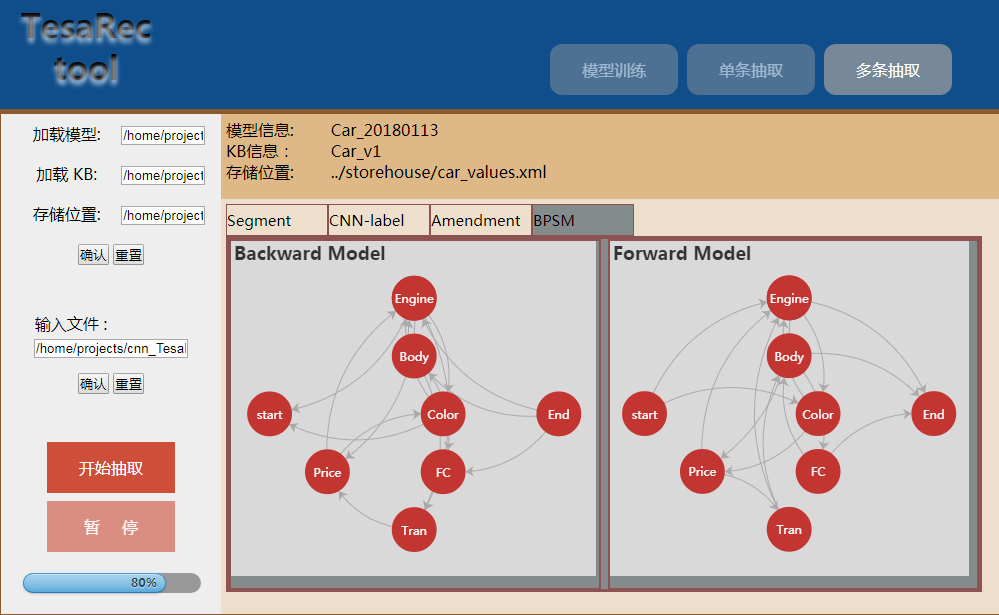
\includegraphics[width=3.5in]{../figures/chap04/BPSM-mul.png}
  }
  \caption{����һ���ļ�}
  \label{fig:mul_record} %% label for entire figure
\end{figure}
